% !TEX root = ../Rulebook.tex

\newpage
\section{Arbitrary Surface Test}

\subsection{Purpose and Focus of the Test}
The purpose of the \iaterm{Arbitrary Surface Test}{AST} is to introduce different kinds of surfaces for the work stations in order to make the operating environment more realistic. In real life scenarios the robot might have to pick objects from different colored or dirty places. Also there could be other industrial items on the surface area that the robot must avoid. This challenge focuses on an advanced perception ability of the robot. \par The main goal of the challenge is to show a reliable and robust vision of the robot during picking operations.

\par
NOTE: The challenges of this test will very likely be transferred to all regular tests from 2019 on!

\subsection{Scenario Environment}
The arena used for this test contains basically all elements as for the Basic Manipulation Test. Additionally to environmental elements (walls, service areas, floor markers, etc.), an object with an arbitrary surface color (see Fig. \ref{ast_example}) will be added to one of the service areas. The referees will prepare the surface on a manipulation zone with a height of 10cm. All geometrical definitions given in Fig.~\ref{fig:manipulation_zone} are considered here too.

\begin{figure}[h!]
\begin{center}
\subfloat[]{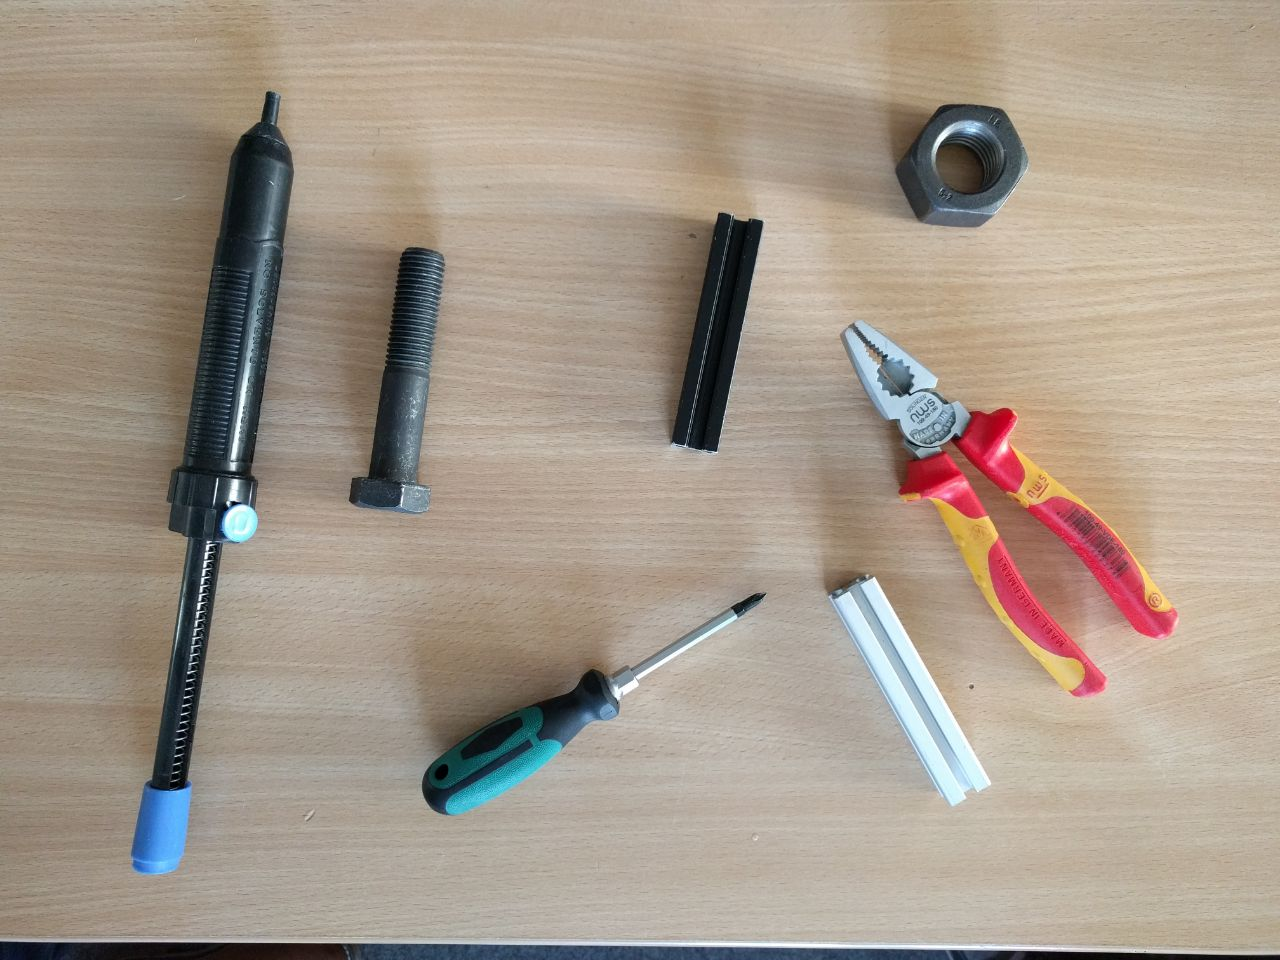
\includegraphics[height = \textwidth/3]{./images/realisticWorkingDeskI}}
\hspace{0.5cm}
\subfloat[]{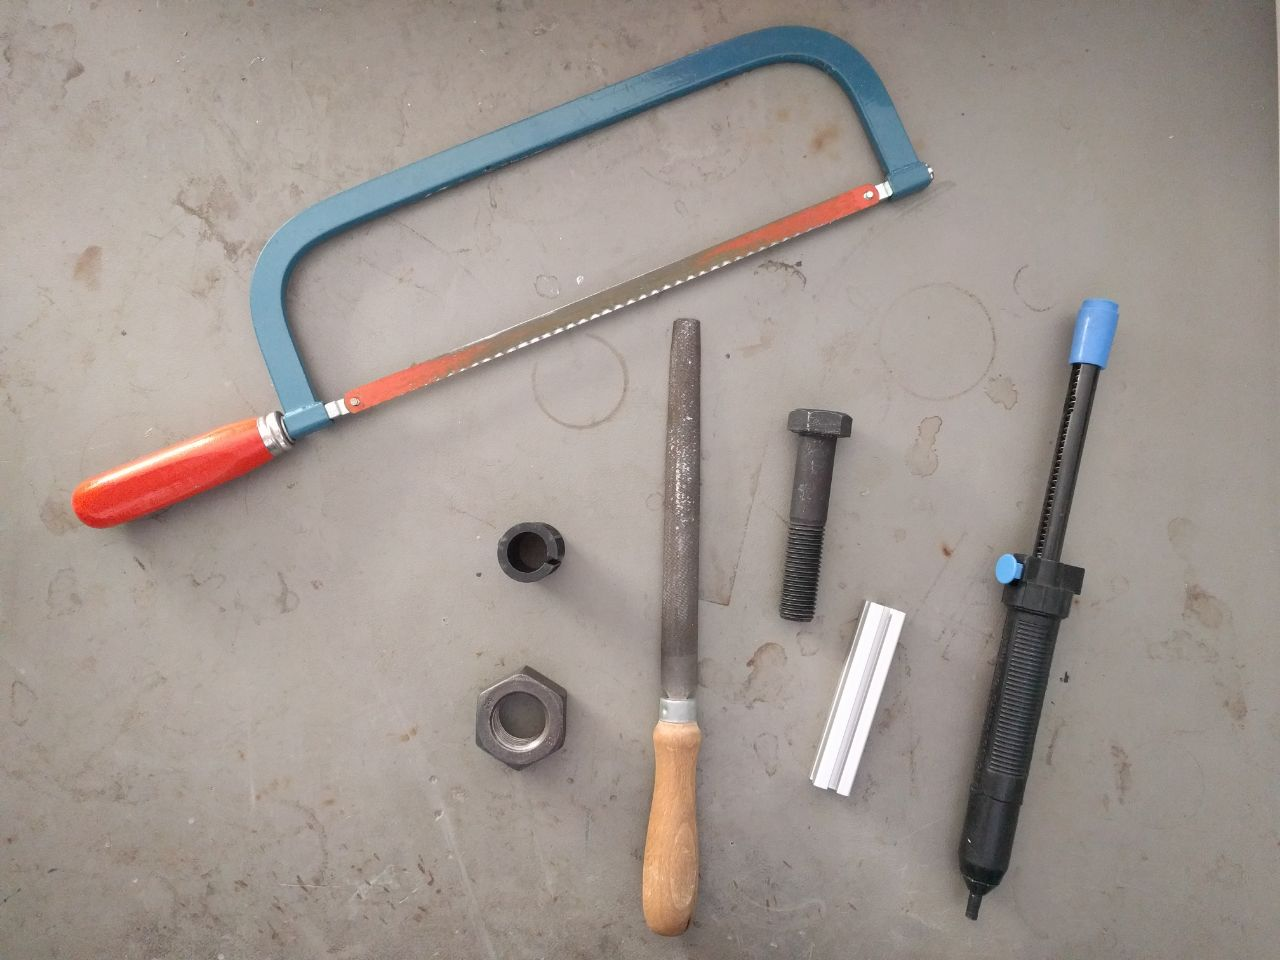
\includegraphics[height = \textwidth/3]{./images/realisticWorkingDeskII}}
\end{center}
\caption{Examplary configuration of the working desks}
\label{ast_example}
\end{figure}


\subsection{Task}
The task consists of navigating to the specified location and then
picking three objects from the service area. There will also be three to five decoy objects that must not be picked up.
\par
The task consists of a sequence of grasp operations. The objective is to pick up all objects specified in the task spec and avoid picking other objects.
\par
The task specification consists of:
\begin{itemize}
	\item[--] The specification of the initial place
	\item[--] A source location, given as place (e.g. \texttt{WS09})
	\item[--] A list of objects to be picked up from the source service area
	\item[--] The specification of a final place for the robot
\end{itemize}


\paragraph{Manipulation Objects}
The manipulation objects used in this test are defined by the instances described in Table~\ref{tab:Instances}.


\subsection{Rules}
The following rules have to be obeyed:

\begin{itemize}
\item A single robot is used.
\item The robot has to start from outside the arena and to end in the final.
\item The order in which the teams have to perform will be determined by a draw.
\item At the beginning of a team's period, the team will get the task specification.
\item A service area counts as successfully reached as defined in Section~\ref{ssec:Navigating}
\item Three objects have to be picked.
\item There will be 3 decoy objects that must not be picked on the service area.
\item A manipulation object counts as successfully grasped as specified in Section~\ref{ssec:GraspingObjects}.
\item The run is over when the robot reached the final place or the designated time has expired.
\end{itemize}

\subsection{Scoring}
\begin{itemize}
\item 100 points are awarded for each correctly and succesfully picked object
\item -50 points for every incorrectly picked object
\item 25 points for reaching the correct service area
\item 25 points for reaching the final position
\end{itemize}
